\documentclass[12pt, a4paper]{article}
\usepackage{../notesheets}
%%%%%%%%%%%%%%%%%%%%%%%%%%%%%%%%%%%%%%%%%%%%%%%%%%
\author{Math 1220}
\title{Notesheet. Section 6.6+7.1: Area between two curves and
  Integration by parts}
\date{}

\begin{document}
\maketitle
\nameline
%%%%%%%%%%%%%%%%%%%%%%%%%%%%%%%%%%%%%%%%%%%%%%%%%%
\begin{thrm}
  If \(f(x) \geq g(x)\) on \([a,b]\), the area of the region between
  \(f\) and \(g\) on \([a,b]\) is given by 
\end{thrm}
\begin{rmk}
  The general formula is given by \(\int_a^b\) \\
\end{rmk}
\vspace{0.5in}
\begin{ex}
  Find the area of the region bounded above by \(f(x) = x\) and bounded below
  by \(g(x) = x^2\) on \([0,1]\). Also can be stated ``find the area of the
  region enclosed by \(f(x) = x\) and \(g(x) = x^2\).''
\end{ex}
\begin{ex}
  Find the area of the region enclosed by \(f(x) = 2x-1\) and \(g(x) =
  x^2-4\).
\end{ex}
\begin{ex}
  Find the area of the following region where the curve is \(y = x^3\):\\
  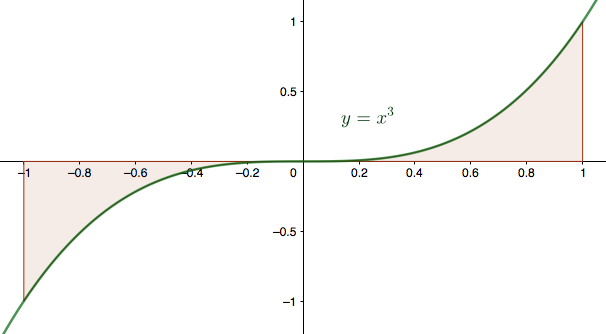
\includegraphics[scale=0.4]{images/area-under-x3}
\end{ex}
\vspace{-1.5in}
\begin{thrm}
  Recall the product rule for derivatives. \[
    \frac{d}{dx}(f(x) \cdot g(x)) = \hspace{3in}
  \]
\end{thrm}
\vspace{0.25in}
\begin{thrm}
  Given functions \(u = f(x)\) and \(v = g(x)\), then \[
    \int u \ dv = \hspace{3in}
  \]
\end{thrm}
\vspace{-0.75in}
\begin{ex}
  Evaluate the following indefinite integrals
  \begin{enumerate}
  \item \(\int x e^x \dx\)
    \vspace{0.75in}
  \item \(\int \frac{\ln x}{x^2} \dx\)
    \vspace{0.75in}
  \item \(\int x \cos(x) \dx\)
  \end{enumerate}
\end{ex}
%%%%%%%%%%%%%%%%%%%%%%%%%%%%%%%%%%%%%%%%%%%%%%%%%% 
\end{document}
